%---------------------------------------------------------------------------%
%-                                                                         -%
%-                           LaTeX Template                                -%
%-                                                                         -%
%---------------------------------------------------------------------------%
%- Copyright (C) Huangrui Mo <huangrui.mo@gmail.com> 
%- ------------------------------------声明---------------------------------%
%- 本模板基于中国科学院大学ucasthesis(mohuangrui版)进行修改,适用于苏州大学硕博
%- (学术/专业)学位论文要求,因时间和能力限制,暂时不支持同等学力版本,且本版本为
%- 非官方版本,各学院专业具体要求不同,可自行修改。
%- 具体使用可参考使用手册
%---------------------------------------------------------------------------%
%->> Document class declaration
%---------------------------------------------------------------------------%
\documentclass[twoside]{Style/sudathesis}%
%- Multiple optional arguments:
%- [oneside] 单面排版,适合作为节省页面的电子版。
%- [twoside] 双面排版,适合作为正式电子版。
%- [print] 预留了装订距离的双面排版,并会将超链接设为黑色,适合作为纸质打印版。
%- 打印前修改为print
%---------------------------------------------------------------------------%
%->> Document settings
%---------------------------------------------------------------------------%
\usepackage[super,list]{Style/artratex}% document settings
%- usage: \usepackage[option1,option2,...,optionN]{artratex}
%- Multiple optional arguments:
%- [<numbers|super|authoryear|alpha>]% 设置引用和参考文献的形式
%- 著者-出版年制(authoryear)为默认选项,不同文献样式和引用样式,如 
%- 著者-出版年制(authoryear)、顺序编码制(numbers)、上标顺序编码制(super)、
%- 字符编码制(alpha)可在 Thesis.tex 中对 artratex.sty 调用实现。
%- 默认使用格式满足学校要求。

\usepackage{Style/artracom}% user defined commands
%---------------------------------------------------------------------------%
%->> Document inclusion
%---------------------------------------------------------------------------%
%\includeonly{Tex/Chap_1,...,Tex/Chap_N}% selected files compilation
%---------------------------------------------------------------------------%
%->> Document content
%---------------------------------------------------------------------------%
%-
%-> Titlepage information
%-
%---------------------------------------------------------------------------%
%->> Titlepage information
%- 	!!!!!!!!!!!!!!!!!!!!!!!!注!!!意!!!!!!!!!!!!!!!!!!!!!!
%- 	!!!!!!!!!!!!!!!!!!!!!!!!注!!!意!!!!!!!!!!!!!!!!!!!!!!
%- !!!请注意,因模板调用要求不同,存在多次设置相同信息问题!!!
%- 	!!!!!!!!!!!!!!!!!!!!!!!!注!!!意!!!!!!!!!!!!!!!!!!!!!!
%- 	!!!!!!!!!!!!!!!!!!!!!!!!注!!!意!!!!!!!!!!!!!!!!!!!!!!
%---------------------------------------------------------------------------%
%-
%-> 中文封面信息
%-
%- 密级:只有涉密论文才填写,编者专业暂未要求;如果需要,可联系编者修改
\schoolid{10285}
\classid{42}
\schoolname[scale=1.0]{name}% 苏州大学
\type{(学术学位)}%学位类型
\schoollogo[scale=1.0]{logo}% 校徽
\title{苏州大学学位论文\LaTeX{}模板 {$~^{\pi}\pi^{\pi}$}}% 论文中文题目文中
\titlea{苏州大学\\学位论文\LaTeX{}模板 {$~^{\pi}\pi^{\pi}$}}% 论文中文题目封面页
\author{莫晃锐}% 论文作者
\advisor{刘青泉}% 指导教师:姓名 专业技术职务 工作单位(两位及以上指导教师使用\\换行)
%\advisor{刘青泉\\刘青泉~研究员~中国科学院理论力学研究所}% 指导教师:姓名 专业技术职务 工作单位
\degree{硕士}% 学位:学士、硕士、博士
\degreetype{理学}% 学位类别:理学、工学、工程、医学等
\major{物理学}% 专业名称
\direction{粒子物理}
\institute{物理与科学技术学院}% 院系名称
\date{2014~年~6~月}% 毕业日期:夏季为6月、冬季为12月
%-
%-> 英文封面信息
%-
\TITLE{\LaTeX{} Thesis Template\\ of \\ Soochow University {$~^{\pi}\pi^{\pi}$}}% 论文英文题目英文封面页
\TITLEA{\LaTeX{} Thesis Template of \\ Soochow University {$~^{\pi}\pi^{\pi}$}}% 论文英文题目中文封面页
\AUTHOR{Mo Huangrui}% 论文作者
\ADVISOR{Professor Liu Qingquan$^a$\\Associate Professor Liu Qingquan$^b$}% 指导教师
\DEGREE{Master}% 学位:Bachelor, Master, Doctor。封面据英文学位名称自动切换,需确保拼写准确
\DEGREETYPE{Natural Science}% 学位类别:Philosophy, Natural Science, Engineering, Economics, Agriculture 等
\MAJOR{Particle Physics and Nuclera Physics}% 专业名称
\INSTITUTE{$^a$School of Physics Science and Technology, Soochow University
	\\$^b$Institute of High Energy Physics, Chinese Academy of Sciences}% 院系名称
\DATE{June, 2014}% 毕业日期:夏季为June、冬季为December
%---------------------------------------------------------------------------%

%-> 盲审封面信息
\titlebr{苏州大学学位论文\LaTeX{}模板 {$~^{\pi}\pi^{\pi}$}\\}% 盲审中文题目
\brstudentnum{2022420000}%申请人学号
\brmajor{物理学}%专业名称
\brdirection{粒子物理学}%研究方向
\brkeywords{苏州大学,学位论文,\LaTeX{}模板\\}%论文关键词

% 设置基本信息
\begin{document}
%-
%-> Frontmatter: title page, abstract, content list, symbol list, preface
%-> Frontmatter:扉页、摘要、内容列表、符号列表、前言
%-
\frontmatter% 调用摘要
%---------------------------------------------------------------------------%
%->> Frontmatter
%---------------------------------------------------------------------------%
%-
%-> 生成封面
%-
%\blindreview%生成盲审封面
\maketitle% 生成中文封面
\MAKETITLE% 生成英文封面
%-
%-> 独创声明
%-
\makedeclaration% 生成声明页
%-
%-> 中文摘要
%-
\abstract{本文是苏州大学学位论文模板sudathesis的使用说明文档。主要内容为介绍\LaTeX{}文档类sudathesis的用法,以及如何使用\LaTeX{}快速高效地撰写学位论文。\textbf{编译前请前往\href{https://github.com/sudathesis/sudathesis/wiki}{\texttt{sudathesis Wiki}} 查看基础介绍}}

\keywords{苏州大学,学位论文,\LaTeX{}模板}% 中文关键词

\absauthor{莫晃锐}
\absadvisor{刘青泉\\莫\quad 锐}%同封面页设置
%-
%-> 注释上方两行,打开下方两行用于盲审
%-
%\absauthor{***}
%\absadvisor{***}%同封面页设置

\makeabstract

%-
%-> 英文摘要
%-
\ABSTRACT{This paper is a help documentation for the \LaTeX{} class sudathesis, which is  a thesis template for Soochow University. The main content is about how to use the sudathesis, as well as how to write thesis efficiently by using \LaTeX{}.}

\KEYWORDS{Soochow University(SUDA), Thesis, \LaTeX{} Template}% 英文关键词

\ABSAUTHOR{Mo Huangrui}
\ABSADVISOR{Liu Qingquan\\Mo rui\\AAAA}%同封面页设置
%-
%-> 注释上方两行,打开下方两行用于盲审
%-
%\ABSAUTHOR{***}
%\ABSADVISOR{***}%同封面页设置

\MAKEABSTRACT


%---------------------------------------------------------------------------%
% 摘要
{% content list region
\linespread{1.2}% 行间距
\intobmk*{\cleardoublepage}{\contentsname}% 添加书签链接
\tableofcontents% 正文目录,不包含中英文摘要
\intobmk*{\cleardoublepage}{\listfigurename}% 添加书签链接
\listoffigures% 插图索引
\intobmk*{\cleardoublepage}{\listtablename}% 添加书签链接
\listoftables% 表格索引
}
\intobmk\chapter*{符号列表}% 显示在书签但不显示在目录

\section*{字符}
\nomenclatureitem[\textbf{Unit}]{\textbf{Symbol}}{\textbf{Description}}
\nomenclatureitem[$\Unit{m^{2} \cdot s^{-2} \cdot K^{-1}}$]{$R$}{the gas constant}
\nomenclatureitem[$\Unit{m^{2} \cdot s^{-2} \cdot K^{-1}}$]{$C_v$}{specific heat capacity at constant volume}
\nomenclatureitem[$\Unit{m^{2} \cdot s^{-2} \cdot K^{-1}}$]{$C_p$}{specific heat capacity at constant pressure}
\nomenclatureitem[$\Unit{m^{2} \cdot s^{-2}}$]{$E$}{specific total energy}
\nomenclatureitem[$\Unit{m^{2} \cdot s^{-2}}$]{$e$}{specific internal energy}
\nomenclatureitem[$\Unit{m^{2} \cdot s^{-2}}$]{$h_T$}{specific total enthalpy}
\nomenclatureitem[$\Unit{m^{2} \cdot s^{-2}}$]{$h$}{specific enthalpy}
\nomenclatureitem[$\Unit{kg \cdot m \cdot s^{-3} \cdot K^{-1}}$]{$k$}{thermal conductivity}
\nomenclatureitem[$\Unit{kg \cdot m^{-1} \cdot s^{-2}}$]{$S_{ij}$}{deviatoric stress tensor}
\nomenclatureitem[$\Unit{kg \cdot m^{-1} \cdot s^{-2}}$]{$\tau_{ij}$}{viscous stress tensor}
\nomenclatureitem[$\Unit{1}$]{$\delta_{ij}$}{Kronecker tensor}
\nomenclatureitem[$\Unit{1}$]{$I_{ij}$}{identity tensor}

\section*{算子}
\nomenclatureitem{\textbf{Symbol}}{\textbf{Description}}
\nomenclatureitem{$\Delta$}{difference}
\nomenclatureitem{$\nabla$}{gradient operator}
\nomenclatureitem{$\delta^{\pm}$}{upwind-biased interpolation scheme}

\section*{缩写}
\nomenclatureitem{CFD}{Computational Fluid Dynamics}
\nomenclatureitem{CFL}{Courant-Friedrichs-Lewy}
\nomenclatureitem{EOS}{Equation of State}
\nomenclatureitem{JWL}{Jones-Wilkins-Lee}
\nomenclatureitem{WENO}{Weighted Essentially Non-oscillatory}
\nomenclatureitem{ZND}{Zel'dovich-von Neumann-Doering}

% 符号表、前言内容
%-
%-> Mainmatter
%-> 正文主体
%-
\mainmatter% 调用正文格式
\chapter{引言}\label{chap:introduction}

\section{研究背景}

多数的苏州大学毕业生在毕业论文排版时选择临时寻找\LaTeX{}模板进行修改,需要耗费不必要的研究修改时间。同时,各类模板修改难易程度不同,效果差异大。在发现中国科学院大学ucasthesis(莫晃锐版)\LaTeX{}模板的优异性后,对其修改适配于苏州大学学位论文编写格式要求,其中大部分底层代码和逻辑继承前者。

当前sudathesis模板满足最新的苏州大学学位论文撰写要求和封面设定。兼顾操作系统:Windows,Linux,MacOS和\LaTeX{}编译引擎:pdflatex,xelatex,lualatex。支持中文书签、中文渲染、中文粗体显示、拷贝PDF中的文本到其他文本编辑器等特性。此外,对模板的文档结构进行了精心设计,撰写了编译脚本提高模板的易用性和使用效率。

sudathesis的目标节省多数人修改\LaTeX{}模板时间,提高学位论文的撰写速度。 同时,sudathesis继承了ucasthesis模板整洁一致的代码结构和扼要的注解。

因为\LaTeX{}使用经验和涉猎层次不一,sudathesis基于\LaTeX{}格式与内容分离的特色,封装底层排版代码,设置简单的接口,降低使用难度,提升使用舒适度。对于初学者而言,使用此模板撰写学位论文本质上不存在技术性的困难。同时,针对\LaTeX{}撰写论文的一些主要难题,如制图、制表、文献索引等,将结合使用情况进行了详细说明,并提供了相应的代码替换方案,具体将在后续章节中进行阐述。


\section{系统要求}\label{sec:system}

\href{https://github.com/sudathesis/sudathesis}{\texttt{sudathesis}} 宏包可以在目前主流的 \href{https://en.wikibooks.org/wiki/LaTeX/Introduction}{\LaTeX{}} 编译系统中使用,如\TeX{}Live和MiK\TeX{}。因C\TeX{}套装已停止维护,\textbf{不再建议使用} (请勿混淆C\TeX{}套装与ctex宏包。C\TeX{}套装是集成了许多\LaTeX{}组件的\LaTeX{}编译系统。 \href{https://ctan.org/pkg/ctex?lang=en}{ctex} 宏包如同sudathesis,是\LaTeX{}命令集,其维护状态活跃,并被主流的\LaTeX{}编译系统默认集成,是几乎所有\LaTeX{}中文文档的核心架构)。推荐的 \href{https://en.wikibooks.org/wiki/LaTeX/Installation}{\LaTeX{}编译系统} 和 \href{https://en.wikibooks.org/wiki/LaTeX/Installation}{\LaTeX{}文本编辑器} 为
\begin{center}
    \begin{tabular}{lcc}
        \hline
        操作系统 & \LaTeX{}编译系统 & \LaTeX{}文本编辑器\\
        \hline
        Linux & \href{https://www.tug.org/texlive/acquire-netinstall.html}{\TeX{}Live Full} & \href{http://texstudio.sourceforge.net/}{TeXstudio} 或 Vim\\
        MacOS & \href{https://www.tug.org/mactex/}{Mac\TeX{} Full} & \href{http://texstudio.sourceforge.net/}{TeXstudio} 或 \href{https://www.texpad.com/}{Texpad for Mac}\\
        Windows & \href{https://www.tug.org/texlive/acquire-netinstall.html}{\TeX{}Live Full} 或 \href{https://miktex.org/download}{MiK\TeX{}} & \href{http://texstudio.sourceforge.net/}{TeXstudio}\\
        \hline
    \end{tabular}
\end{center}

\LaTeX{}编译系统,如\TeX{}Live(Mac\TeX{}为针对MacOS的\TeX{}Live),用于提供编译环境,\LaTeX{}文本编辑器 (如Texmaker) 用于编辑\TeX{}源文件。请从各软件官网下载安装程序,勿使用不明程序源。\textbf{\LaTeX{}编译系统和\LaTeX{}编辑器分别安装成功后,即完成了\LaTeX{}的系统配置},无需其他手动干预和配置。若系统原带有旧版的\LaTeX{}编译系统并想安装新版,请\textbf{先卸载干净旧版再安装新版}。

\section{问题反馈}

sudathesis基于ucasthesis对苏州大学毕业论文要求进行排版适配,未对底层逻辑和代码进行大篇幅修改,因此大多数常见问题可以前往ucasthesis的 \href{https://github.com/mohuangrui/ucasthesis/wiki/%E5%B8%B8%E8%A7%81%E9%97%AE%E9%A2%98}{问题反馈} 查看。
对于修改的sudathesis模板中出现的问题可以反馈至\href{https://github.com/sudathesis/sudathesis/issues}{sudathesis Issues},在力所能及的情况下将及时修改完善。

\section{模板下载}

\begin{center}
    \href{https://github.com/sudathesis/sudathesis}{Github/sudathesis}: \url{https://github.com/sudathesis/sudathesis}
\end{center}
 %引言
\chapter{模板文件介绍}\label{chap:texintro}

基于文件分类管理原则便于修改与操作的属性,本模板对sudathesis的框架和文件体系进行分类系统管理。对于初次使用者,\LaTeX{}编译后的众多的文件目录不知所云,在阅读完模板文件介绍后,将会轻松使用。除此之外,\LaTeX{}的使用方法可以通过阅读相关资料如\LaTeX{} Wikibook \citep{wikibook2014latex} 增添使用技巧。


\section{安装与操作}

\begin{enumerate}
    \item 安装软件:根据所用操作系统和章节~\ref{sec:system}中的信息安装\LaTeX{}编译环境。
    \item 获取模板:下载 \href{https://github.com/sudathesis/sudathesis}{\texttt{sudathesis}} 模板并解压。sudathesis模板不仅提供了相应的类文件,同时也提供了包括参考文献等在内的完成学位论文的一切要素,所以,下载时,推荐下载整个sudathesis文件夹,而不是单独的文档类。
    \item 编译模板:
        \begin{enumerate}
            \item Windows:双击运行artratex.bat脚本。
            \item Linux或MacOS: { \verb|terminal| -> \verb|chmod +x ./artratex.sh| -> \verb|./artratex.sh xa|}
            \item \color{red}任意系统:都可使用\LaTeX{}编辑器打开Thesis.tex文件并选择xelatex编译引擎进行编译。\\
            具体编译流程为 Xelatex -> Bibtex -> Xelatex -> Xelatex,即后文所提方法。
        \end{enumerate}
    \item 错误处理:若编译中遇到了问题,请先查看“常见问题”(章节~\ref{sec:qa})。
\end{enumerate}

编译完成即可获得本PDF说明文档。而这也完成了学习使用sudathesis撰写论文的一半进程。

\section{文档目录简介}

\subsection{Thesis.tex}

Thesis.tex为主文档,其设计和规划了论文的整体框架,通过对其的阅读可以了解整个论文框架的搭建。

\subsection{编译脚本}

\begin{itemize}
    \item Windows:双击Dos脚本artratex.bat可得全编译后的PDF文档,其存在是为了帮助不了解\LaTeX{}编译过程的初学者跨过编译这第一道坎,请勿通过邮件传播和接收此脚本,以防范Dos脚本的潜在风险。
    \item Linux或MacOS:在terminal中运行
        \begin{itemize}
            \item \verb|./artratex.sh xa|:获得全编译后的PDF文档
            \item \verb|./artratex.sh x|:快速编译,不会生成文献引用
        \end{itemize}
\end{itemize}

全编译指运行 \verb|Xelatex+Bibtex+Xelatex+Xelatex| 以正确生成所有的引用链接,如目录,参考文献及引用等。在写作过程中若无添加新的引用,则可用快速编译,即只运行一遍\LaTeX{}编译引擎以减少编译时间。

\subsection{Tmp文件夹}

运行编译脚本后,编译所生成的文档皆存于Tmp文件夹内,包括编译得到的PDF文档,其存在是为了保持工作空间的整洁,因为好的心情是很重要的。

\subsection{Style文件夹}

包含ucasthesis文档类的定义文件和配置文件,通过对它们的修改可以实现特定的模版设定。

\begin{enumerate}
    \item sudathesis.cls:文档类定义文件,论文的最核心的格式即通过它来定义的。
    \item sudathesis.cfg:文档类配置文件,设定如目录显示为“目~录”而非“目录”。
    \item artratex.sty: 常用宏包及文档设定,如参考文献样式、文献引用样式、页眉页脚设定等。这些功能具有开关选项,常只需在Thesis.tex中进行启用即可,一般无需修改artratex.sty本身。
    \item artracom.sty:自定义命令以及添加宏包的推荐放置位置。
\end{enumerate}

\subsection{Tex文件夹}

文件夹内为论文的所有实体内容,正常情况下,这也是\textbf{使用sudathesis撰写学位论文时,主要关注和修改的一个位置,注:所有文件都必须采用UTF-8编码,否则编译后将出现乱码文本},详细分类介绍如下:

\begin{itemize}
    \item Frontinfo.tex:为论文中英文封面信息。\textbf{论文封面会根据英文学位名称如Bachelor,Master,Doctor, Postdoctor 自动切换为相应的格式}。
    \item Frontmatter.tex:为论文前言内容如中英文摘要等。
    \item Mainmatter.tex:索引需要出现的Chapter。开始写论文时,可以只索引当前章节,以快速编译查看,当论文完成后,再对所有章节进行索引即可。
    \item Chap{\_}xxx.tex:为论文主体的各章,可根据需要添加和撰写。\textbf{添加新章时,可拷贝一个已有的章文件再重命名,以继承文档的 UTF8 编码}。
    \item Appendix.tex:为附录内容。
    \item Backmatter.tex:为发表文章信息和致谢部分等。
\end{itemize}

\subsection{Img文件夹}

用于放置论文中所需要的图类文件,支持格式有:.eps, .jpg, .png, .pdf。其中,\verb|logo.png|苏州大学校徽、\verb|name.png|苏州大学校名图片格式。若图片众多,也可为各章节图片建立子目录;但若命名规则合理,图片查询亦是十分方便。

\subsection{Biblio文件夹}

\begin{enumerate}
    \item ref.bib:参考文献信息库。
\end{enumerate}


 %第一章
\chapter{模板使用说明}\label{chap:guide}

\section{字体、图表、数学公式、参考文献等功能}

\subsection{文档内字体切换方法}
具体使用代码可查看tex文档下方示例,也可以前往\href{https://github.com/sudathesis/sudathesis/wiki/%E5%AD%97%E4%BD%93%E5%AD%97%E5%8F%B7#%E5%B8%B8%E7%94%A8%E5%AD%97%E4%BD%93%E4%BF%AE%E6%94%B9}{常用字体修改}查看。
\begin{itemize}
	\item 宋体:论文模板 或 \textrm{论文模板}
	\item 粗宋体:{\bfseries 论文模板} 或 \textbf{论文模板}
	\item 黑体:{\sffamily 论文模板} 或 \textsf{论文模板}
	\item 粗黑体:{\bfseries\sffamily 论文模板} 或 \textsf{\bfseries 论文模板}
	\item 仿宋:{\ttfamily 论文模板} 或 \texttt{论文模板}
	\item 粗仿宋:{\bfseries\ttfamily 论文模板} 或 \texttt{\bfseries 论文模板}
	\item 楷体:{\itshape 论文模板} 或 \textit{论文模板}
	\item 粗楷体:{\bfseries\itshape 论文模板} 或 \textit{\bfseries 论文模板}
\end{itemize}

\subsection{表格}

请见表~\ref{tab:sample}。
\begin{table}[!htbp]
	\bicaption{这是一个样表。}{This is a sample table.}
	\label{tab:sample}
	\centering
	\footnotesize% fontsize
	\setlength{\tabcolsep}{4pt}% column separation
	\renewcommand{\arraystretch}{1.2}%row space 
	\begin{tabular}{lcccccccc}
		\hline
		行号 & \multicolumn{8}{c}{跨多列的标题}\\
		%\cline{2-9}% partial hline from column i to column j
		\hline
		Row 1 & $1$ & $2$ & $3$ & $4$ & $5$ & $6$ & $7$ & $8$\\
		Row 2 & $1$ & $2$ & $3$ & $4$ & $5$ & $6$ & $7$ & $8$\\
		Row 3 & $1$ & $2$ & $3$ & $4$ & $5$ & $6$ & $7$ & $8$\\
		Row 4 & $1$ & $2$ & $3$ & $4$ & $5$ & $6$ & $7$ & $8$\\
		\hline
	\end{tabular}
\end{table}

基础制表案例及制表方法请见 \href{https://github.com/sudathesis/sudathesis/wiki#%E8%A1%A8%E6%A0%BC%E8%AE%BE%E7%BD%AE}{sudathesis表格设置}表格常用形式。制图制表的更多范例,请见 \href{https://en.wikibooks.org/wiki/LaTeX/Tables}{WiKibook Tables}。

\subsection{图片插入}

论文中图片的插入通常分为单图和多图,下面分别加以介绍:

单图插入:假设插入名为\verb|c06h06|(后缀可以为.jpg、.png、.pdf,下同)的图片,其效果如图~\ref{fig:c06h06}。
\begin{figure}[!htbp]
	\centering
	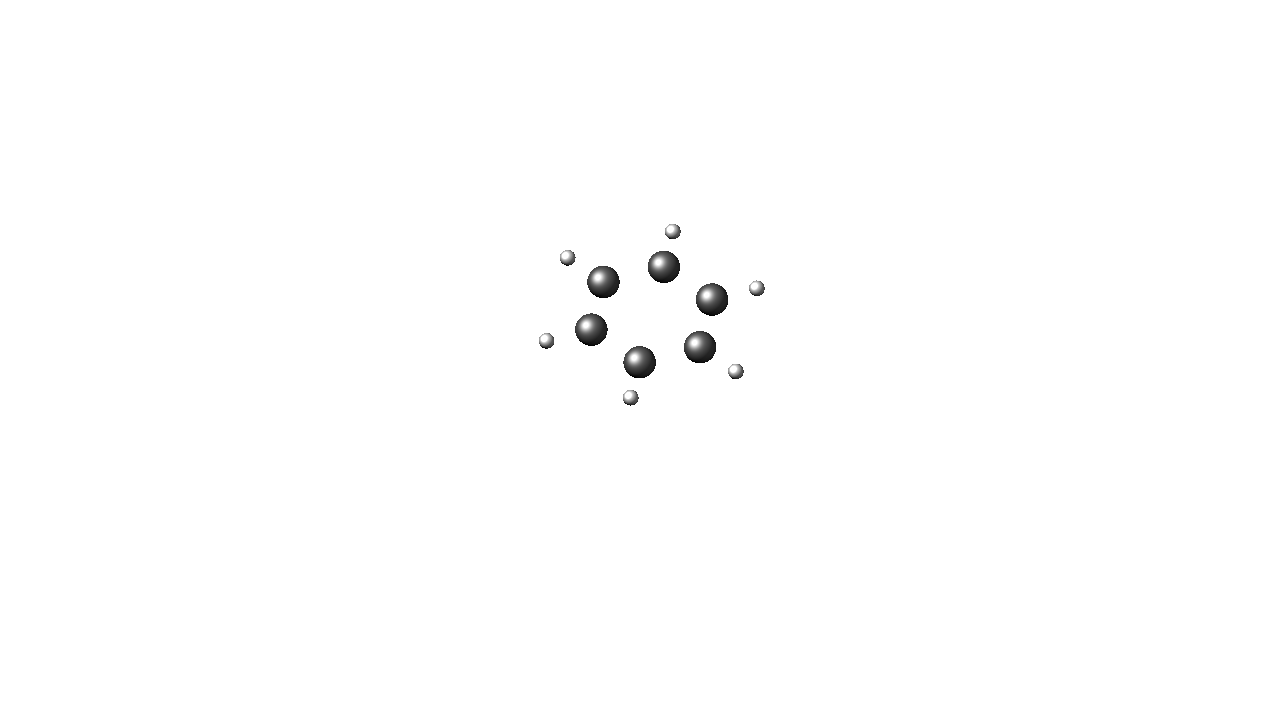
\includegraphics[width=0.40\textwidth]{c06h06}
	\caption{Q判据等值面图,同时测试一下一个很长的标题,比如这真的是一个很长很长很长很长很长很长很长很长的标题。}
	\label{fig:c06h06}
\end{figure}

如果插图的空白区域过大,以图片\verb|c06h06|为例,自动裁剪如图~\ref{fig:c06h06_trim}。
\begin{figure}[!htbp]
	\centering
	%trim option's parameter order: left bottom right top
	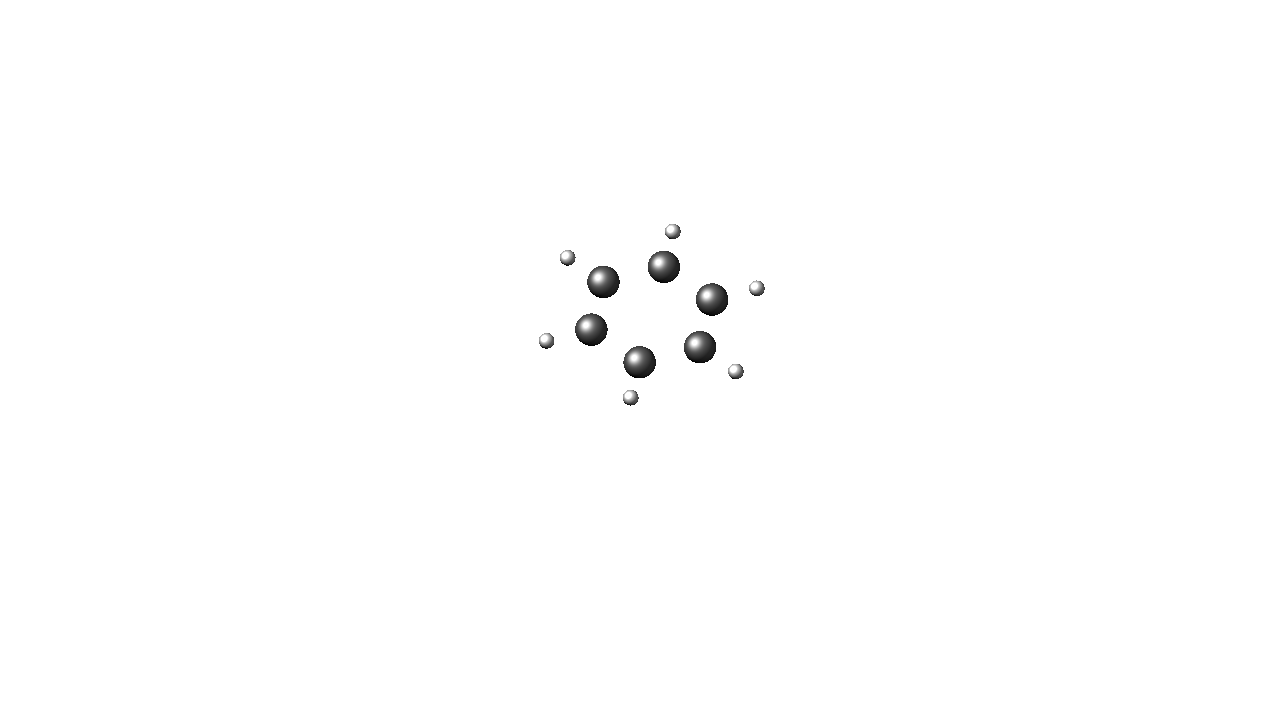
\includegraphics[trim = 60mm 80mm 60mm 60mm, clip, width=0.40\textwidth]{c06h06}
	\caption{激波圆柱作用。}
	\label{fig:c06h06_trim}
\end{figure}

多图的插入如图~\ref{fig:oaspl},多图不应在子图中给文本子标题,只要给序号,并在主标题中进行引用说明。
\begin{figure}[!htbp]
	\centering
	\begin{subfigure}[b]{0.35\textwidth}
		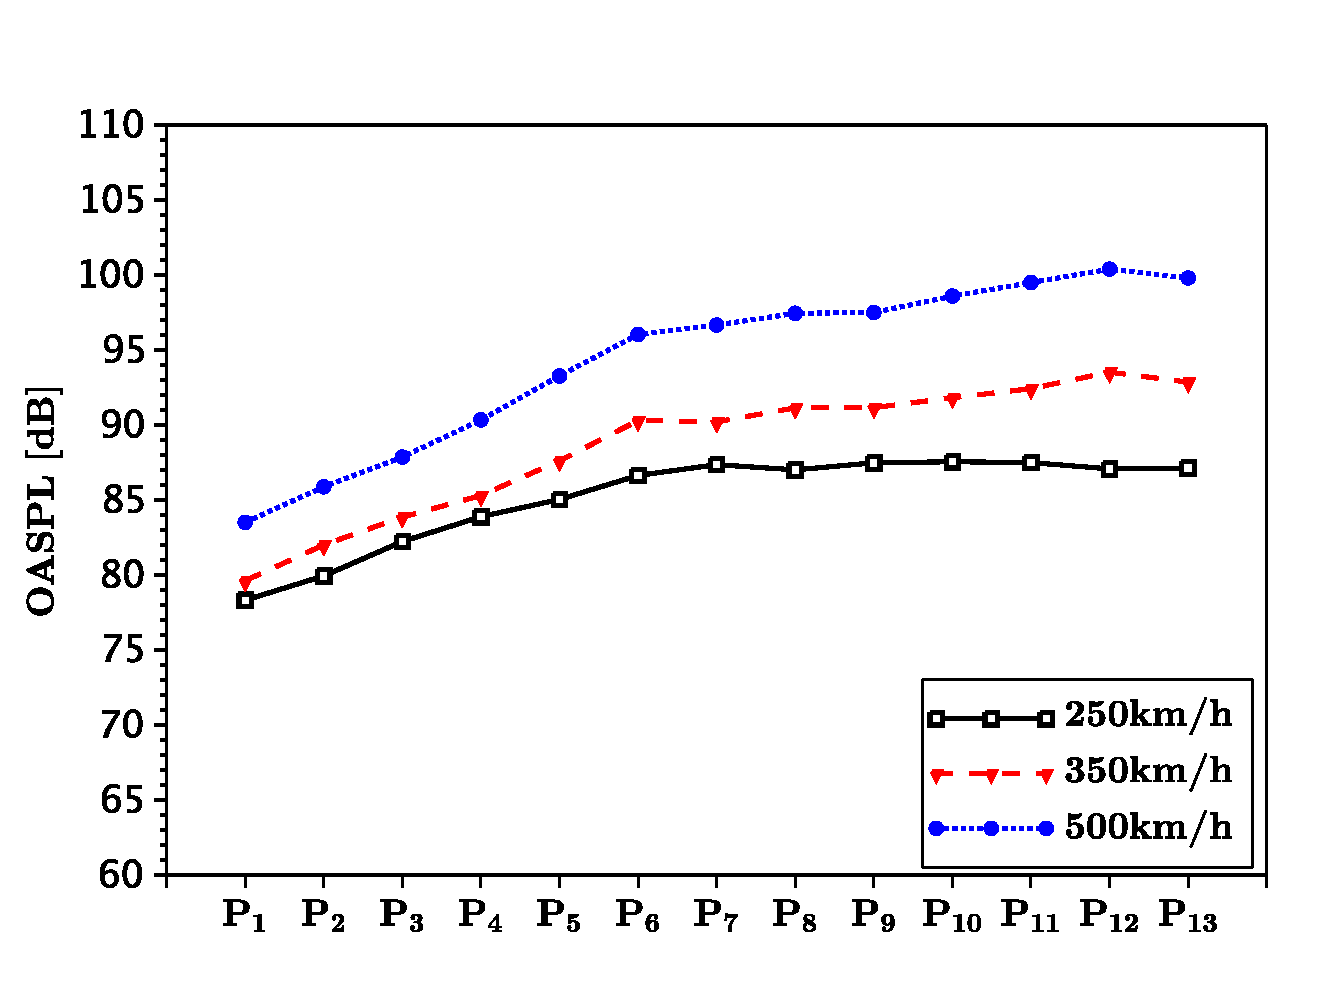
\includegraphics[width=\textwidth]{oaspl_a}
		\caption{}
		\label{fig:oaspl_a}
	\end{subfigure}%
	~% add desired spacing
	\begin{subfigure}[b]{0.35\textwidth}
		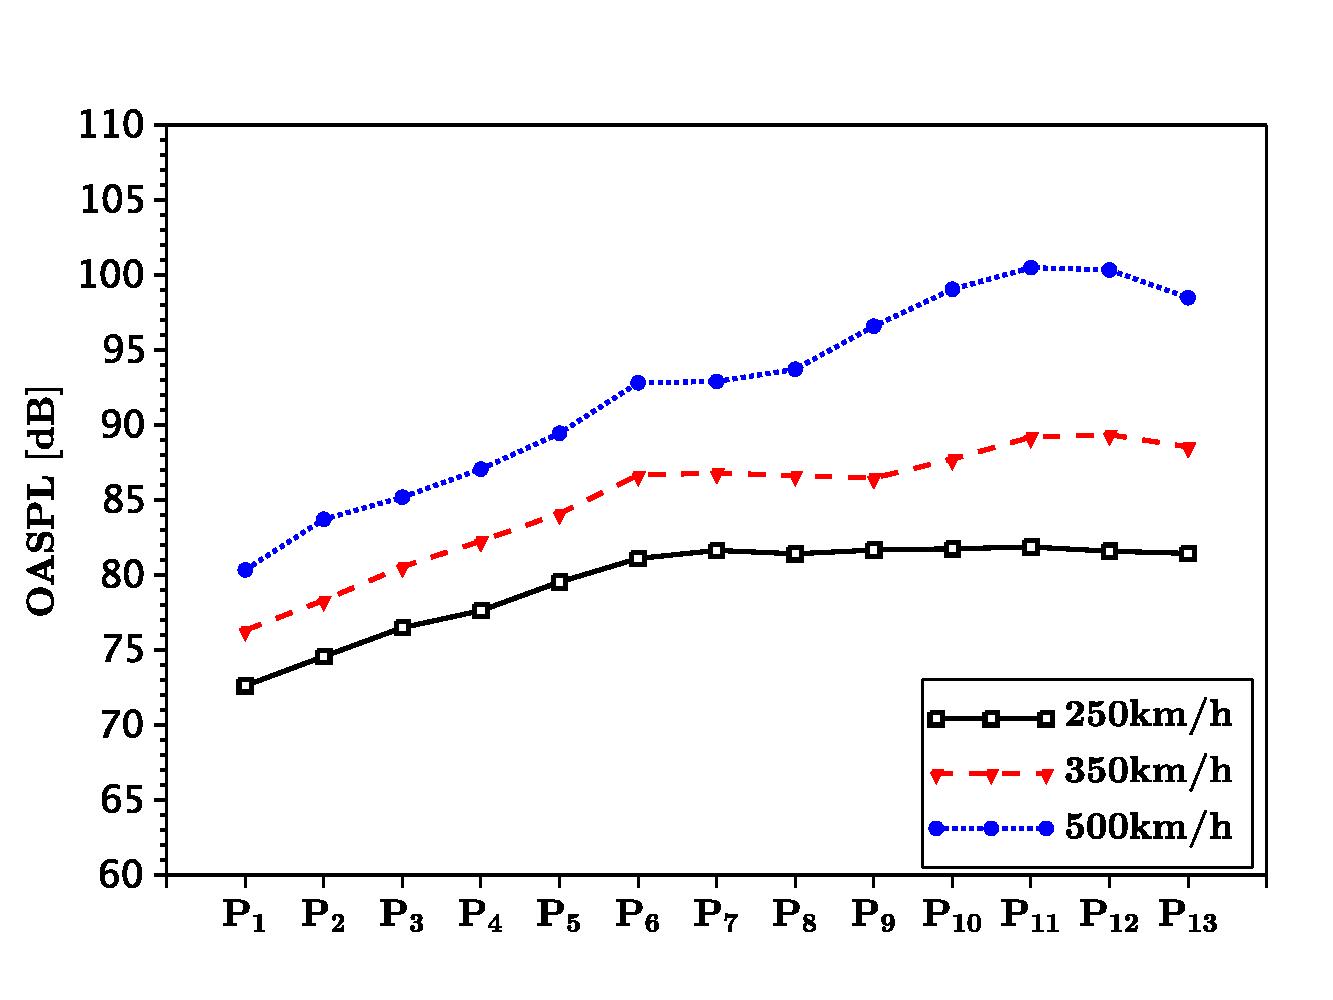
\includegraphics[width=\textwidth]{oaspl_b}
		\caption{}
		\label{fig:oaspl_b}
	\end{subfigure}
	\\% line break
	\begin{subfigure}[b]{0.35\textwidth}
		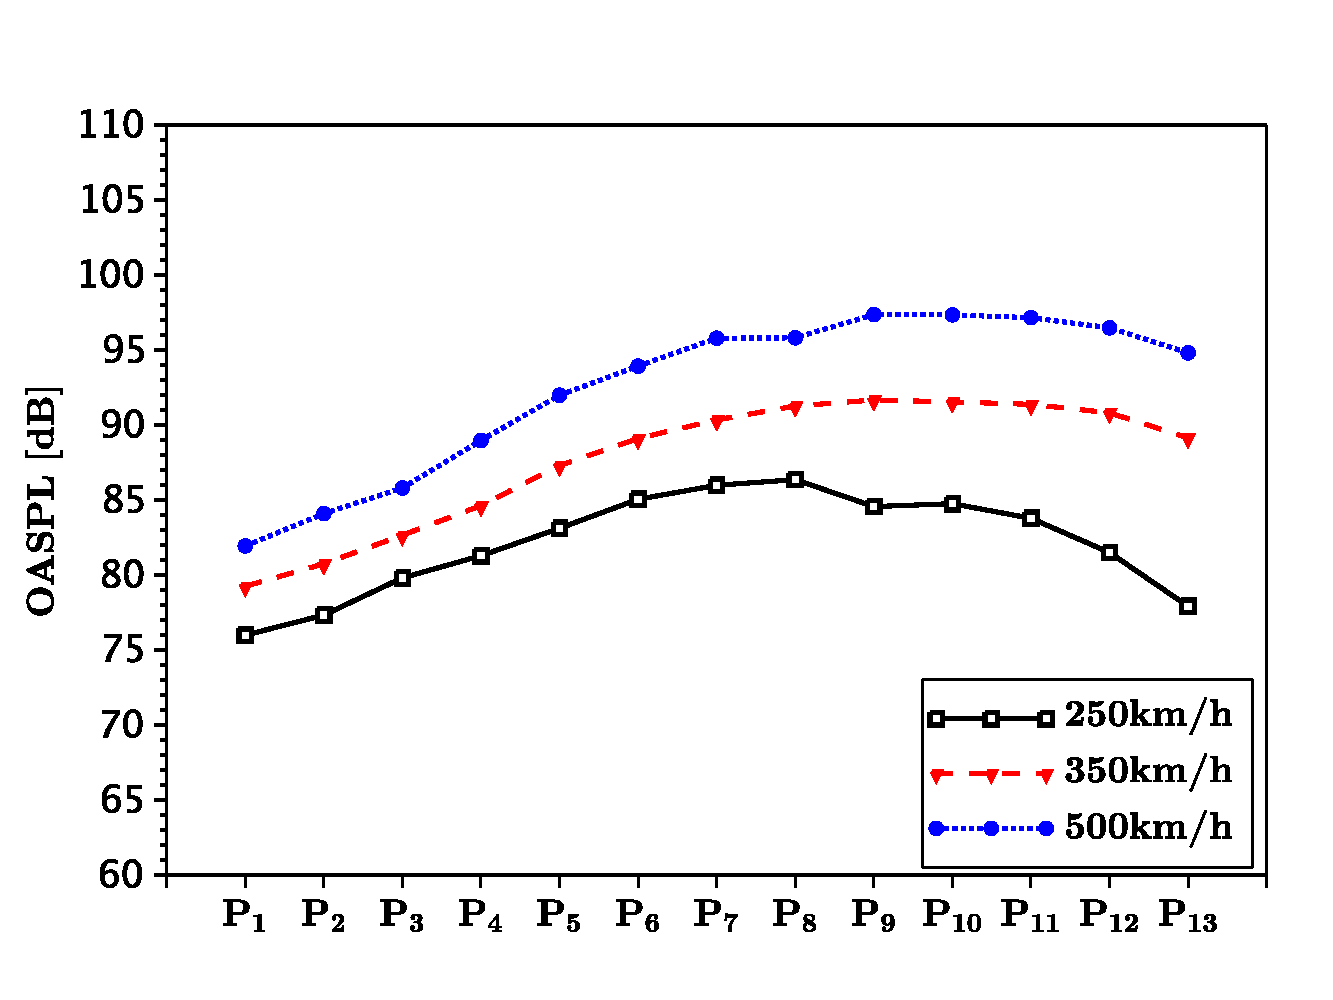
\includegraphics[width=\textwidth]{oaspl_c}
		\caption{}
		\label{fig:oaspl_c}
	\end{subfigure}%
	~% add desired spacing
	\begin{subfigure}[b]{0.35\textwidth}
		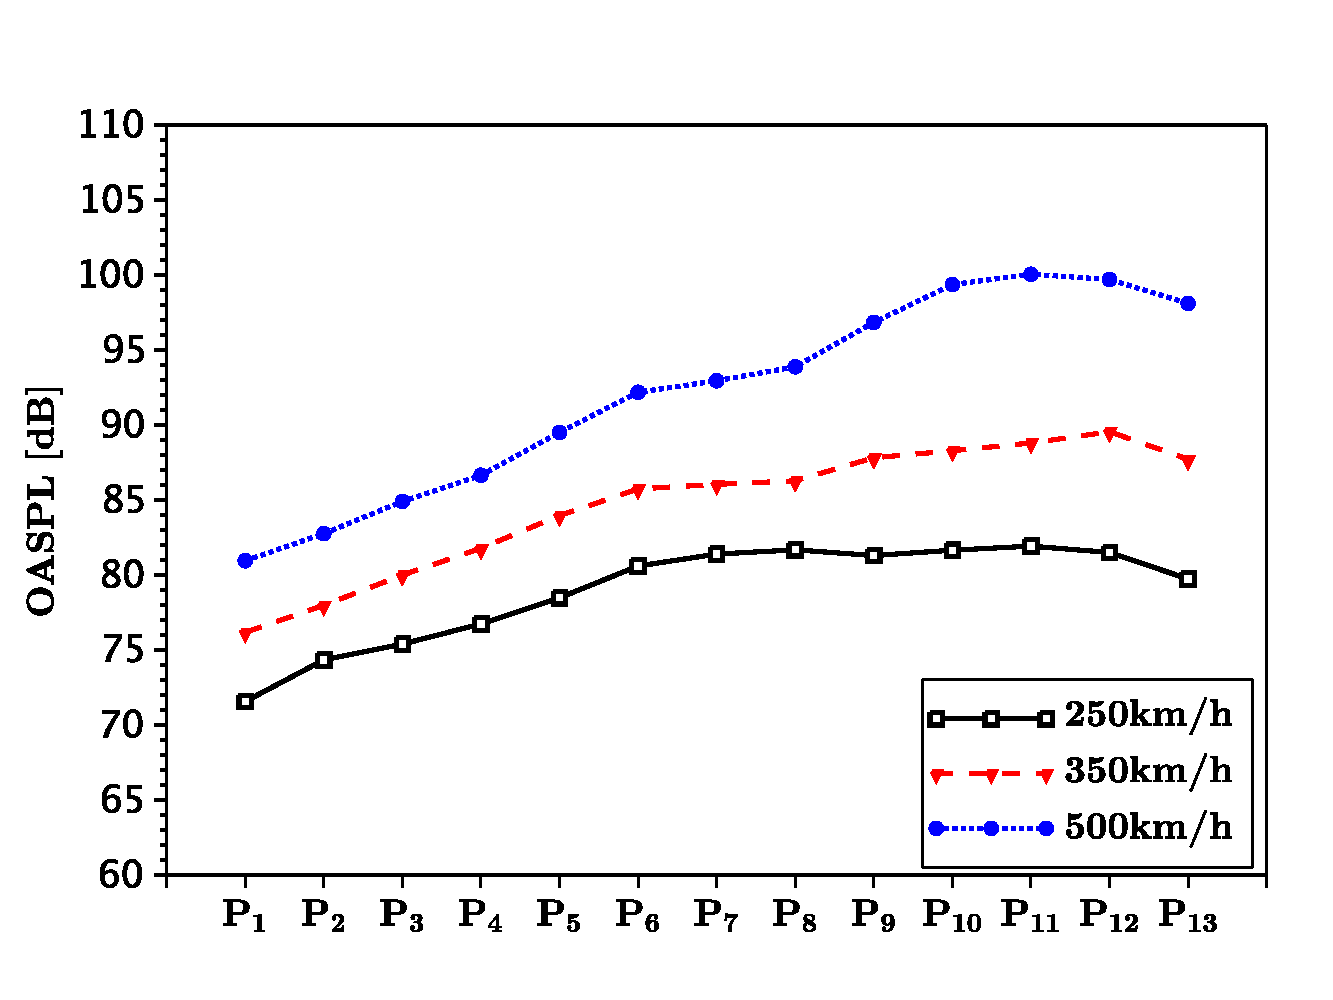
\includegraphics[width=\textwidth]{oaspl_d}
		\caption{}
		\label{fig:oaspl_d}
	\end{subfigure}
	\caption{总声压级。(a) 这是子图说明信息,(b) 这是子图说明信息,(c) 这是子图说明信息,(d) 这是子图说明信息。}
	\label{fig:oaspl}
\end{figure}


\subsection{数学公式}

比如Navier-Stokes方程(方程~\eqref{eq:ns}):
\begin{equation} \label{eq:ns}
    \adddotsbeforeeqnnum%
    \begin{cases}
        \frac{\partial \rho}{\partial t} + \nabla\cdot(\rho\Vector{V}) = 0 \ \mathrm{times\ math\ test: 1,2,3,4,5}, 1,2,3,4,5\\
        \frac{\partial (\rho\Vector{V})}{\partial t} + \nabla\cdot(\rho\Vector{V}\Vector{V}) = \nabla\cdot\Tensor{\sigma} \ \text{times text test: 1,2,3,4,5}\\
        \frac{\partial (\rho E)}{\partial t} + \nabla\cdot(\rho E\Vector{V}) = \nabla\cdot(k\nabla T) + \nabla\cdot(\Tensor{\sigma}\cdot\Vector{V})
    \end{cases}
\end{equation}
\begin{equation}
    \adddotsbeforeeqnnum%
    \frac{\partial }{\partial t}\int\limits_{\Omega} u \, \mathrm{d}\Omega + \int\limits_{S} \unitVector{n}\cdot(u\Vector{V}) \, \mathrm{d}S = \dot{\phi}
\end{equation}
\[
    \begin{split}
        \mathcal{L} \{f\}(s) &= \int _{0^{-}}^{\infty} f(t) e^{-st} \, \mathrm{d}t, \ 
        \mathscr{L} \{f\}(s) = \int _{0^{-}}^{\infty} f(t) e^{-st} \, \mathrm{d}t\\
        \mathcal{F} {\bigl (} f(x+x_{0}) {\bigr )} &= \mathcal{F} {\bigl (} f(x) {\bigr )} e^{2\pi i\xi x_{0}}, \ 
        \mathscr{F} {\bigl (} f(x+x_{0}) {\bigr )} = \mathscr{F} {\bigl (} f(x) {\bigr )} e^{2\pi i\xi x_{0}}
    \end{split}
\]

数学公式常用命令请见 \href{https://en.wikibooks.org/wiki/LaTeX/Mathematics}{WiKibook Mathematics}。artracom.sty中对一些常用数据类型如矢量矩阵等进行了封装,这样的好处是如有一天需要修改矢量的显示形式,只需单独修改artracom.sty中的矢量定义即可实现全文档的修改。

\subsection{数学环境}

\begin{axiom}
   这是一个公理。 
\end{axiom}
\begin{theorem}
   这是一个定理。 
\end{theorem}
\begin{lemma}
   这是一个引理。 
\end{lemma}
\begin{corollary}
   这是一个推论。 
\end{corollary}
\begin{assertion}
   这是一个断言。 
\end{assertion}
\begin{proposition}
   这是一个命题。 
\end{proposition}
\begin{proof}
    这是一个证明。
\end{proof}
\begin{definition}
    这是一个定义。
\end{definition}
\begin{example}
    这是一个例子。
\end{example}
\begin{remark}
    这是一个注。
\end{remark}


\subsection{算法}

如见算法~\ref{alg:euclid},详细使用方法请参见文档 \href{https://ctan.org/pkg/algorithmicx?lang=en}{algorithmicx}。

\begin{algorithm}[!htbp]
    \small
    \caption{Euclid's algorithm}\label{alg:euclid}
    \begin{algorithmic}[1]
        \Procedure{Euclid}{$a,b$}\Comment{The g.c.d. of a and b}
        \State $r\gets a\bmod b$
        \While{$r\not=0$}\Comment{We have the answer if r is 0}
        \State $a\gets b$
        \State $b\gets r$
        \State $r\gets a\bmod b$
        \EndWhile\label{euclidendwhile}
        \State \textbf{return} $b$\Comment{The gcd is b}
        \EndProcedure
    \end{algorithmic}
\end{algorithm}

\subsection{参考文献引用}

参考文献引用过程以实例进行介绍,假设需要引用名为"Document Preparation System"的文献,步骤如下:

1)使用Google Scholar搜索Document Preparation System,在目标条目下点击Cite,展开后选择Import into BibTeX打开此文章的BibTeX索引信息,将它们copy添加到ref.bib文件中(此文件位于Biblio文件夹下)。

2)索引第一行 \verb|@article{lamport1986document,|中 \verb|lamport1986document| 即为此文献的label (\textbf{中文文献也必须使用英文label},一般遵照:姓氏拼音+年份+标题第一字拼音的格式),想要在论文中索引此文献,有两种索引类型:

文本类型:\verb|\citet{lamport1986document}|。正如此处所示 \citet{lamport1986document}; 

括号类型:\verb|\citep{lamport1986document}|。正如此处所示 \citep{lamport1986document}。

\textbf{多文献索引用英文逗号隔开}:

\verb|\citep{lamport1986document, chu2004tushu, chen2005zhulu}|。正如此处所示 \citep{lamport1986document, chu2004tushu, chen2005zhulu}

更多例子如:

\citet{walls2013drought} 根据 \citet{betts2005aging} 的研究,首次提出...。其中关于... \citep{walls2013drought, betts2005aging},是当前中国...得到迅速发展的研究领域 \citep{chen1980zhongguo, bravo1990comparative}。引用同一著者在同一年份出版的多篇文献时,在出版年份之后用
英文小写字母区别,如:\citep{yuan2012lana, yuan2012lanb, yuan2012lanc} 和 \citet{yuan2012lana, yuan2012lanb, yuan2012lanc}。同一处引用多篇文献时,按出版年份由近及远依次标注。例如 \citep{chen1980zhongguo, stamerjohanns2009mathml, hls2012jinji, niu2013zonghe}。

使用著者-出版年制(authoryear)式参考文献样式时,中文文献必须在BibTeX索引信息的 \textbf{key} 域(请参考ref.bib文件)填写作者姓名的拼音,才能使得文献列表按照拼音排序。参考文献表中的条目(不排序号),先按语种分类排列,语种顺 序是:中文、日文、英文、俄文、其他文种。然后,中文按汉语拼音字母顺序排列,日文按第一著者的姓氏笔画排序,西文和 俄文按第一著者姓氏首字母顺序排列。如中 \citep{niu2013zonghe}、日 \citep{Bohan1928}、英 \citep{stamerjohanns2009mathml}、俄 \citep{Dubrovin1906}。

如此,即完成了文献的索引,请查看下本文档的参考文献一章,看看是不是就是这么简单呢?是的,就是这么简单!

不同文献样式和引用样式,如著者-出版年制(authoryear)、顺序编码制(numbers)、上标顺序编码制(super)可在Thesis.tex中对artratex.sty调用实现,详见 \href{https://github.com/mohuangrui/ucasthesis/wiki}{ucasthesis 知识小站之文献样式}

%若在上标顺序编码制(super)模式下,希望在特定位置将上标改为嵌入式标,可使用 \citetns{niu2013zonghe,stamerjohanns2009mathml} 和 \citepns{niu2013zonghe,stamerjohanns2009mathml}。

参考文献索引的更多知识,请见 \href{https://en.wikibooks.org/wiki/LaTeX/Bibliography_Management}{WiKibook Bibliography}。\nocite{*}% 使文献列表显示所有参考文献(包括未引用文献)

\section{常见使用问题}\label{sec:qa}

\begin{enumerate}
    \item 模板在发布前,已在Windows,Linux,MacOS系统上测试通过。下载模板后,若编译出现错误,则请见 \href{https://github.com/mohuangrui/ucasthesis/wiki}{ucasthesis知识小站} 的 \href{https://github.com/mohuangrui/ucasthesis/wiki/%E7%BC%96%E8%AF%91%E6%8C%87%E5%8D%97}{编译指南}。

    \item 模板文档的编码为UTF-8编码。所有文件都必须采用UTF-8编码,否则编译后生成的文档将出现乱码文本。若出现文本编辑器无法打开文档或打开文档乱码的问题,请检查编辑器对UTF-8编码的支持。如果使用WinEdt作为文本编辑器(\textbf{不推荐使用}),应在其Options -> Preferences -> wrapping选项卡下将两种Wrapping Modes中的内容:
        
        TeX;HTML;ANSI;ASCII|DTX...
        
        修改为:TeX;\textbf{UTF-8|ACP;}HTML;ANSI;ASCII|DTX...
        
        同时,取消Options -> Preferences -> Unicode中的Enable ANSI Format。

    \item 推荐选择xelatex或lualatex编译引擎编译中文文档。编译脚本的默认设定为xelatex编译引擎。你也可以选择不使用脚本编译,如直接使用 \LaTeX{}文本编辑器编译。注:\LaTeX{}文本编辑器编译的默认设定为pdflatex编译引擎,若选择xelatex或lualatex编译引擎,请进入下拉菜单选择。为正确生成引用链接和参考文献,需要进行\textbf{全编译}。

    \item Texmaker使用简介
        \begin{enumerate}
            \footnotesize
            \item 使用 Texmaker “打开 (Open)” Thesis.tex。
            \item 菜单 “选项 (Options)” -> “设置当前文档为主文档 (Define as Master Document)”
            \item 菜单 “自定义 (User)” -> “自定义命令 (User Commands)” -> “编辑自定义命令 (Edit User Commands)” -> 左侧选择 “command 1”,右侧 “菜单项 (Menu Item)” 填入 Auto Build -> 点击下方“向导 (Wizard)” -> “添加 (Add)”: xelatex + bibtex + xelatex + xelatex + pdf viewer -> 点击“完成 (OK)”
            \item 使用 Auto Build 编译带有未生成引用链接的源文件,可以仅使用 xelatex 编译带有已经正确生成引用链接的源文件。
            \item 编译完成,“查看(View)” PDF,在PDF中 “ctrl+click” 可链接到相对应的源文件。
        \end{enumerate}
    
    \item 模版的设计可能地考虑了适应性。致谢等所有条目都是通过最为通用的

        \verb+\chapter{item name}+  and \verb+\section*{item name}+

        来显式实现的 (请观察Backmatter.tex),从而可以随意添加,放置,和修改,如同一般章节。对于图表目录名称则可在ucasthesis.cfg中进行修改。

    \item 设置文档样式: 在artratex.sty中搜索关键字定位相应命令,然后修改
        \begin{enumerate}
            \item 正文行距:启用和设置 \verb|\linespread{1.5}|,默认1.5倍行距。
            \item 参考文献行距:修改 \verb|\setlength{\bibsep}{0.0ex}|
            \item 目录显示级数:修改 \verb|\setcounter{tocdepth}{2}|
            \item 文档超链接的颜色及其显示:修改 \verb|\hypersetup|
        \end{enumerate}


\end{enumerate}


 %第二章
%- 请继续添加
%-
%-> Appendix
%-
\cleardoublepage%
\appendix% 调用附录格式
\chapter{苏州大学学位论文撰写要求}

学位论文是研究生科研工作成果的集中体现,是评判学位申请者学术水平、授予其学位的主要依据,是科研领域重要的文献资料。根据《科学技术报告、学位论文和学术论文的编写格式》(GB/T 7713-1987)、《学位论文编写规则》(GB/T 7713.1-2006)和《文后参考文献著录规则》(GB7714—87)等国家有关标准,结合苏州大学(以下简称“苏大”)的实际情况,特制订本规定。

\section{论文无附录者无需附录部分}

\section{测试公式编号 \texorpdfstring{$\Lambda,\lambda,\theta,\bar{\Lambda},\sqrt{S_{NN}}$}{$\textLambda,\textlambda,\texttheta,\bar{\textLambda},\sqrt{S_{NN}}$}} \label{sec:testmath}

\begin{equation} \label{eq:appedns}
    \adddotsbeforeeqnnum%
    \begin{cases}
        \frac{\partial \rho}{\partial t} + \nabla\cdot(\rho\Vector{V}) = 0\\
        \frac{\partial (\rho\Vector{V})}{\partial t} + \nabla\cdot(\rho\Vector{V}\Vector{V}) = \nabla\cdot\Tensor{\sigma}\\
        \frac{\partial (\rho E)}{\partial t} + \nabla\cdot(\rho E\Vector{V}) = \nabla\cdot(k\nabla T) + \nabla\cdot(\Tensor{\sigma}\cdot\Vector{V})
    \end{cases}
\end{equation}
\begin{equation}
    \adddotsbeforeeqnnum%
    \frac{\partial }{\partial t}\int\limits_{\Omega} u \, \mathrm{d}\Omega + \int\limits_{S} \unitVector{n}\cdot(u\Vector{V}) \, \mathrm{d}S = \dot{\phi}
\end{equation}
\[
    \begin{split}
        \mathcal{L} \{f\}(s) &= \int _{0^{-}}^{\infty} f(t) e^{-st} \, \mathrm{d}t, \ 
        \mathscr{L} \{f\}(s) = \int _{0^{-}}^{\infty} f(t) e^{-st} \, \mathrm{d}t\\
        \mathcal{F} {\bigl (} f(x+x_{0}) {\bigr )} &= \mathcal{F} {\bigl (} f(x) {\bigr )} e^{2\pi i\xi x_{0}}, \ 
        \mathscr{F} {\bigl (} f(x+x_{0}) {\bigr )} = \mathscr{F} {\bigl (} f(x) {\bigr )} e^{2\pi i\xi x_{0}}
    \end{split}
\]

mathtext: $A,F,L,2,3,5,\sigma$, mathnormal: $A,F,L,2,3,5,\sigma$, mathrm: $\mathrm{A,F,L,2,3,5,\sigma}$.

mathbf: $\mathbf{A,F,L,2,3,5,\sigma}$, mathit: $\mathit{A,F,L,2,3,5,\sigma}$, mathsf: $\mathsf{A,F,L,2,3,5,\sigma}$.

mathtt: $\mathtt{A,F,L,2,3,5,\sigma}$, mathfrak: $\mathfrak{A,F,L,2,3,5,\sigma}$, mathbb: $\mathbb{A,F,L,2,3,5,\sigma}$.

mathcal: $\mathcal{A,F,L,2,3,5,\sigma}$, mathscr: $\mathscr{A,F,L,2,3,5,\sigma}$, boldsymbol: $\boldsymbol{A,F,L,2,3,5,\sigma}$.

vector: $\Vector{\sigma, T, a, F, n}$, unitvector: $\unitVector{\sigma, T, a, F, n}$

matrix: $\Matrix{\sigma, T, a, F, n}$, unitmatrix: $\unitMatrix{\sigma, T, a, F, n}$

tensor: $\Tensor{\sigma, T, a, F, n}$, unittensor: $\unitTensor{\sigma, T, a, F, n}$ 

\section{测试生僻字}

霜蟾盥薇曜灵霜颸妙鬘虚霩淩澌菀枯菡萏泬寥窅冥毰毸濩落霅霅便嬛岧峣瀺灂姽婳愔嫕飒纚棽俪緸冤莩甲摛藻卮言倥侗椒觞期颐夜阑彬蔚倥偬澄廓簪缨陟遐迤逦缥缃鹣鲽憯懔闺闼璀错媕婀噌吰澒洞阛闠覼缕玓瓑逡巡諓諓琭琭瀌瀌踽踽叆叇氤氲瓠犀流眄蹀躞赟嬛茕頔璎珞螓首蘅皋惏悷缱绻昶皴皱颟顸愀然菡萏卑陬纯懿犇麤掱暒 墌墍墎墏墐墒墒墓墔墕墖墘墖墚墛坠墝增墠墡墢墣墤墥墦墧墨墩墪樽墬墭堕墯墰墱墲坟墴墵垯墷墸墹墺墙墼墽垦墿壀壁壂壃壄壅壆坛壈壉壊垱壌壍埙壏壐壑壒压壔壕壖壗垒圹垆壛壜壝垄壠壡坜壣壤壥壦壧壨坝塆圭嫶嫷嫸嫹嫺娴嫼嫽嫾婳妫嬁嬂嬃嬄嬅嬆嬇娆嬉嬊娇嬍嬎嬏嬐嬑嬒嬓嬔嬕嬖嬗嬘嫱嬚嬛嬜嬞嬟嬠嫒嬢嬣嬥嬦嬧嬨嬩嫔嬫嬬奶嬬嬮嬯婴嬱嬲嬳嬴嬵嬶嬷婶嬹嬺嬻嬼嬽嬾嬿孀孁孂娘孄孅孆孇孆孈孉孊娈孋孊孍孎孏嫫婿媚嵭嵮嵯嵰嵱嵲嵳嵴嵵嵶嵷嵸嵹嵺嵻嵼嵽嵾嵿嶀嵝嶂嶃崭嶅嶆岖嶈嶉嶊嶋嶌嶍嶎嶏嶐嶑嶒嶓嵚嶕嶖嶘嶙嶚嶛嶜嶝嶞嶟峤嶡峣嶣嶤嶥嶦峄峃嶩嶪嶫嶬嶭崄嶯嶰嶱嶲嶳岙嶵嶶嶷嵘嶹岭嶻屿岳帋巀巁巂巃巄巅巆巇巈巉巊岿巌巍巎巏巐巑峦巓巅巕岩巗巘巙巚帠帡帢帣帤帨帩帪帬帯帰帱帲帴帵帷帹帺帻帼帽帾帿幁幂帏幄幅幆幇幈幉幊幋幌幍幎幏幐幑幒幓幖幙幚幛幜幝幞帜幠幡幢幤幥幦幧幨幩幪幭幮幯幰幱庍庎庑庖庘庛庝庠庡庢庣庤庥庨庩庪庬庮庯庰庱庲庳庴庵庹庺庻庼庽庿廀厕廃厩廅廆廇廋廌廍庼廏廐廑廒廔廕廖廗廘廙廛廜廞庑廤廥廦廧廨廭廮廯廰痈廲廵廸廹廻廼廽廿弁弅弆弇弉弖弙弚弜弝弞弡弢弣弤弨弩弪弫弬弭弮弰弲弪弴弶弸弻弼弽弿彖彗彘彚彛彜彝彞彟彴彵彶彷彸役彺彻彽彾佛徂徃徆徇徉后徍徎徏径徒従徔徕徖徙徚徛徜徝从徟徕御徢徣徤徥徦徧徨复循徫旁徭微徯徰徱徲徳徴徵徶德徸彻徺忁忂惔愔忇忈忉忔忕忖忚忛応忝忞忟忪挣挦挧挨挩挪挫挬挭挮挰掇授掉掊掋掍掎掐掑排掓掔掕挜掚挂掜掝掞掟掠采探掣掤掦措掫掬掭掮掯掰掱掲掳掴掵掶掸掹掺掻掼掽掾掿拣揁揂揃揅揄揆揇揈揉揊揋揌揍揎揑揓揔揕揖揗揘揙揤揥揦揧揨揫捂揰揱揲揳援揵揶揷揸揻揼揾揿搀搁搂搃搄搅搇搈搉搊搋搌搎搏搐搑搒摓摔摕摖摗摙摚摛掼摝摞摠摡斫斩斮斱斲斳斴斵斶斸旪旫旮旯晒晓晔晕晖晗晘晙晛晜晞晟晠晡晰晣晤晥晦晧晪晫晬晭晰晱晲晳晴晵晷晸晹晻晼晽晾晿暀暁暂暃暄暅暆暇晕晖暊暋暌暍暎暏暐暑暒暓暔暕暖暗旸暙暚暛暜暝暞暟暠暡暣暤暥暦暧暨暩暪暬暭暮暯暰昵暲暳暴暵
% 附录内容
%-
%-> Backmatter: bibliography, glossary, index
%-> Backmatter: 参考书目、词汇表、索引
%-
\backmatter% initialize the environment
\intotoc*{\cleardoublepage}{\bibname}% 添加书签链接
\artxifstreq{\artxbib}{bibtex}{% 支持 bibtex
    \bibliography{Biblio/ref}% bibliography
}{%
    \printbibliography% bibliography
}

%---------------------------------------------------------------------------%
%->> Backmatter
%---------------------------------------------------------------------------%
\chapter[致谢]{致\quad 谢}\chaptermark{致\quad 谢}% syntax: \chapter[目录]{标题}\chaptermark{页眉}
%\thispagestyle{noheaderstyle}% 如果需要移除当前页的页眉
%\pagestyle{noheaderstyle}% 如果需要移除整章的页眉

非常感谢ucasthesis的作者mohuangrui,他的ucasthesis模板代码逻辑清晰,结构简单,为我调整适配苏州大学学位论文编写要求的\LaTeX{}模板sudathesis相关工作节省很多时间。同时,对于mohuangrui所提及感谢的所有人也表示感谢。基于他们的智慧、辛勤付出和非凡工作,\LaTeX{}知识薄弱的我勉强完成对苏州大学学位论文\LaTeX{}模板sudathesis的修改工作。此外在自己的使用\LaTeX{}过程中,离不开众多在开源社区提供优秀教程和有效指导的贡献者,在此一致表示感谢!





\chapter{作者简历及攻读学位期间发表的学术论文与研究成果}

\textbf{本科生无需此部分}。

\section*{作者简历:}


\subsection*{ucasthesis作者}

莫晃锐,湖南省湘潭县人,中国科学院力学研究所硕士研究生。

\section*{已发表(或正式接受)的学术论文:}

{
\setlist[enumerate]{}% restore default behavior
\begin{enumerate}[nosep]
    \item ucasthesis: A LaTeX Thesis Template for the University of Chinese Academy of Sciences, 2014.
\end{enumerate}
}

\section*{申请或已获得的专利:}

(无专利时此项不必列出)

\section*{参加的研究项目及获奖情况:}

可以随意添加新的条目或是结构。

\cleardoublepage[plain]% 让文档总是结束于偶数页,可根据需要设定页眉页脚样式,如 [noheaderstyle]
%---------------------------------------------------------------------------%
% 致谢和成果总结
\end{document}
%---------------------------------------------------------------------------%

